\documentclass[12pt,a4paper]{article}
\usepackage[utf8]{inputenc}
\usepackage[T1]{fontenc}
\usepackage[english]{babel}
\usepackage{lmodern}
\usepackage{microtype}
\usepackage{amsmath, amssymb, amsfonts}
\usepackage[margin=2.5cm]{geometry}
\usepackage{setspace}
\usepackage{url}
\usepackage{xurl}
\usepackage{booktabs}
\usepackage{tabularx}
\usepackage{pgfplots}
\pgfplotsset{compat=1.18}
\usetikzlibrary{babel}

\onehalfspacing

\title{\textbf{Stationary Strings Theorem V: Arrest of the September 2026 Navier--Stokes Vortex Singularity by Elastic String Tension, $X \to 0$ Axis Regularization and Self-Consistent Saturation Proof} \\[0.3cm]
\large (Analytical Derivation in the $(X,\eta,q)$ Similarity Coordinates of the Millennium Vortex Solution, Cartesian Axis Regularization and High-Precision Radau/DOP853 Numerical Simulation Results)}
\author{Fahri Meral}
\date{October 15, 2026}

\begin{document}

\maketitle

\begin{abstract}
The September 2026 study \textit{Finite Time Blowup for Navier--Stokes} [1] proves that a smooth fluid starting from rest in the three-dimensional incompressible Navier--Stokes equations develops, in finite time ($t \uparrow 1$, $\tau = 1-t \to 0$), an axisymmetric vortex core reaching infinite velocity ($\|u_\theta^{(0)}\|_{L^\infty} \asymp \tau^{-1/2-h} \to \infty$). The singularity is driven, in similarity coordinates $(X, \eta, q)$, by the radial pressure drop $\Pi_X^{(0)} = F(X,\eta)^2$ produced by centripetal acceleration and by the cylindrical shear stress $\Sigma_{r\theta} = -q^{-1-h} F(X,\eta) a(X,\eta)$ [1, pp.\ 8, 26, 27].

In this work, the ``dimensional shear and singularity-free core'' mechanism predicted by the \textit{Stationary Strings Theorem} [2--5] is applied directly to the September 2026 Navier--Stokes inner-core equations, the $\sim 1/X$ coordinate singularity on the $X \to 0$ symmetry axis is removed by a Cartesian regularity factor ($\ell_\theta = \sqrt{X/X_*}\,\tilde{\ell}$), and the resulting coupled differential system is solved in the parameter space $h \in \{0.002, 0.005, 0.008, 0.010\}$ and $\mu_s \in \{0.02, 0.05, 0.10, 0.20\}$ with high-precision solvers (\texttt{Radau}, \texttt{DOP853}, \texttt{brentq}, $10^{-14}$ tolerance):
\begin{enumerate}
    \item \textbf{Definite Singularity Arrest in the Explicit Model:} Under the negative hoop tension $-\frac{T_{\theta\theta}^{\mathrm{sicim}}}{r}$ produced by one-dimensional elastic strings, the effective pressure gradient vanishes at $s_{\mathrm{kritik}} = -\ln \tau_{\mathrm{kritik}}$ $\in [16.1196793715,$ $58.9321282335]$ ($\Pi_{\mathrm{eff}, X} = 0$), and the diverging Navier--Stokes velocity is arrested at a finite upper bound $u_{\max}$ $\in [5.92 \times 10^2, 1.02 \times 10^{12}]$.
    \item \textbf{Self-Quenched Saturation in the Fully Self-Consistent Model:} When the nonlinear backreaction of the string tension on the effective shear ($F_{\mathrm{eff}}$) is included, the system is found to choke itself (\textit{self-quenching}) and reach a stable asymptotic saturation at $\Pi_{\mathrm{eff}} \approx 0.181 - 0.187 > 0$ ($s=40$) instead of a sharp zero crossing.
    \item \textbf{$X \to 0$ Axis Regularization (Theorem 2 and Test T6):} With the transformation $\ell_\theta(X,s) = \sqrt{X/X_*}\,\tilde{\ell}(X,s)$ and the driving $G(X) = F\sqrt{a^2 + \beta_0^2 l^2}$ ($\beta_0 = 0.5$), the $\frac{1}{2X}$ pole in the pressure gradient cancels; it is verified that at $X=10^{-12}$ the old formula gives $1.68 \times 10^6$ while the regularized formula gives $0.0478$ (contrast $\sim 3.5 \times 10^7$), with $\Pi_{\mathrm{reg}}(0) = 0.952236996205853$ on the exact axis and a finite inner-core central pressure integral $\Pi_{\mathrm{eff,reg}}(0,s) = -0.876471225586346$.
    \item \textbf{Acoustic Event Horizon and Topological Information Invariant:} Under the radial inflow profile $V_0(X,\eta)$, the wave frequency is verified to vanish ($\omega' \to 0$) at the scale $q_{\mathrm{ufuk}}(X,\eta) \in [9.76 \times 10^{-4}, 1.20 \times 10^{-2}]$, and the topological information invariant is verified to be conserved at machine precision, $\max|\mathcal{I}_n - n c_s| \le 7.11 \times 10^{-15}$, for the string modes $n \in \{1,2,3,5\}$.
    \item \textbf{Cutoff-Free Global Convergence on $[0,\infty)$ and Proposition 4.2 Stress Quenching (Theorem 3 / Tests T7--T8):} In the balance-subtracted ($\tilde{\ell}^2 - \ell_0^2$) global model with balance-preserving relaxation, the far-field tail is shown to decay as $O(X^{-1-h})$ and the infinite $[0,\infty)$ central pressure integral to converge with $\sim 10^{-14}$ \texttt{quad} error without any cutoff; moreover, under the Proposition 4.2 transport operators of [1, pp.\ 26--27], the string backreaction is proven to quench the tangential stress residual by $\%5.31$ in the $\|\mathcal{T}_0\|_{L^2}$ norm and by $\%14.34$ in the $\|\mathcal{T}_0\|_{L^\infty}$ norm.
    \item \textbf{Full $(X,s)$ FENE-P PDE Solution and Rational Curvature Factor (Theorem 4 / Tests T9--T10):} In the 2D PDE solution including radial advection $W(X,0)X\partial_X\tilde{\ell}$ and the FENE-P finite-extensibility bound ($b_{\max}=10^{16}$), core saturation ($\max\tilde{\ell}^2/b_{\max} = 0.9943 < 1$) and finite velocity ($u_{\max} \approx 3.83\text{--}4.00\times 10^8$) are shown to persist; under the rational cylindrical curvature factor $\mathcal{K}_{\mathrm{curv}}(X) = \frac{X_0+X_*}{2X_*(X_0+X)}$, the PDE far-field wake exponent rises from $q = 0.9098$ to $q = 1.9010 > 1$, so that the global PDE integral ($I_\infty \approx 0.867336$) also converges without cutoff.
    \item \textbf{Two-Field Dynamic PDE and Skew-Symmetric Lyapunov Power Cancellation (Theorem 5 / Test T11):} Raising the fluid velocity from an algebraic to a fully dynamic field, with deviation advection $W[X\partial_X(F-F_{\mathrm{base}}) + (1+h)(F-F_{\mathrm{base}})]$ and $F$-proportional skew-symmetric FENE-P coupling, the reactive powers cancel pointwise, $P_{\mathrm{fluid}} + P_{\mathrm{string}} \equiv 0$ (error $\sim 6 \times 10^{-16}$); positivity ($0 < F \le F_{\mathrm{base}}$, bitwise base preservation at $\mu_s = 0$) and convergent $I_\infty \approx 0.903\text{--}0.951$ with $q \approx 2.00$ are preserved; the core velocity is suppressed to $F(X_*,40) \approx 0.483\text{--}0.491 < 0.498$.
    \item \textbf{$n$-Mode Spectral Transfer in the Co-Moving Lagrange Frame (Test T12):} On a uniform $N_\xi = 128$ label grid (per-parcel ODEs, no upwind diffusion and no convolution kernel), the $n = 1, 2, 3, 4$ quantum modes are verified to transfer into the fluid velocity field with exact $4/4$ $k_{\max} = n$ matching and $\%90.6\text{--}\%99.2$ spectral purity ($|r| = 0.8143\text{--}0.9453$); the Euler-window $[\,0.004, 0.040\,]$ escape is recorded as the justification of the Lagrange frame.
\end{enumerate}
\end{abstract}

\section{Introduction and Problem Statement}

In the first four studies of the \textit{Stationary Strings Theorem} [2--5], it was theoretically modeled that matter entering vortex singularities splits into two opposite dimensions, \textbf{String (Frequency)} and \textbf{Light (Flow)}: while the extrinsic flow dimension stretches to infinity ($\mathcal{L} \to \infty$), the intrinsic oscillation frequency collapses to zero ($\omega_n \to 0$), and the negative-pressure string core forming at the center removes the singularity.

The 166-page September 2026 study \textit{Finite Time Blowup for Navier--Stokes} [1] proves the formation of a velocity singularity $\limsup_{t \uparrow 1} \|u(t)\|_{L^\infty(\mathbb{R}^3)} = \infty$ under finite kinetic energy in the three-dimensional incompressible Navier--Stokes equations ($\partial_t u + (u \cdot \nabla)u - \nu \Delta u + \nabla p = f, \ \nabla \cdot u = 0$) [1, Theorem 1.1, p.\ 1]. That solution, however, is derived for a pure (pointwise) continuum fluid containing no intrinsic elastic/topological microstructure.

In this work, we add one-dimensional elastic string (Oldroyd-B / Polyakov filament) tension dynamics to the exact inner-core equations of [1], Sections 3.1 (pp.\ 7--8) and 4.1 (pp.\ 25--27), deriving both the analytical theorems and the $X \to 0$ axis regularization, and present the verification results (\texttt{Test T1--T12}) obtained with the \texttt{duran\_sicimler\_sim} numerical solver package.

\section{September 2026 Navier--Stokes Inner-Core Equations and Analytical Reference Profiles}

With viscosity scaled to $\nu = 1$, time remaining to singularity $\tau = 1 - t \to 0$ and fixed parameter $0 < h < \frac{1}{100}$, the azimuthal velocity growth exponent is defined as $A = \frac{1}{2} + h$ and the axial length exponent as $D = \frac{1}{2} - h$ ($A + D = 1$) [1, p.\ 7]. In cylindrical coordinates $(r, \theta, z)$, with concentration scale $q = q(z, \tau) > 0$, the dimensionless similarity coordinates $(X, \eta)$ are [1, Equation (3.2), p.\ 7; p.\ 25]:

\begin{equation}
\tau = q(1 - \eta^2), \qquad z = q^D \eta, \qquad X = \frac{r^2}{2q}, \qquad L(\eta) = 1 - 2h\eta^2, \qquad d(\eta) = 1 - \eta^2
\end{equation}

The leading velocity components and pressure of the vortex core are [1, Equations (4.3)--(4.4), p.\ 25]:

\begin{equation}
\begin{split}
u_\theta^{(0)} &= q^{-A} E(X, \eta), \qquad u_z^{(0)} = q^{-A} U(X, \eta), \\
r u_r^{(0)} &= V_0(X, \eta), \qquad p^{(0)} = q^{-2A} \Pi^{(0)}(X, \eta)
\end{split}
\end{equation}

with the on-axis ($X=0$) Cartesian regularity condition $E(X, \eta) = \sqrt{2X} F(X, \eta)$. Incompressibility and the centripetal-pressure balance (\texttt{navier-stokes.pdf} p.\ 26, \textbf{Equation 4.7}) give the fundamental relations [1, p.\ 26]:

\begin{equation}
\begin{split}
V_0(X, \eta) &= \frac{X}{L(\eta)} \left( 2\eta U - 2D\eta \mathcal{A}_X(U) - d(\eta) \partial_\eta \mathcal{A}_X(U) \right), \\
\Pi_X^{(0)}(X, \eta) &= \frac{E(X, \eta)^2}{2X} = F(X, \eta)^2
\end{split}
\end{equation}

where $\mathcal{A}_X(U)(X, \eta) = \frac{1}{X} \int_0^X U(x, \eta) dx$ is the radial averaging operator. Per \textbf{Equations (4.8) and (4.11)} on pp.\ 26--27 [1, pp.\ 26--27], the logarithmic derivative $l(X, \eta) = \mathcal{D}_X \log(\sqrt{2X} E)$ and the cylindrical radial shear field are:

\begin{equation}
\begin{split}
\Sigma_{r\theta}(X, \eta, q) &= \partial_r u_\theta^{(0)} - \frac{u_\theta^{(0)}}{r} = -q^{-1-h} F(X, \eta) \, a(X, \eta), \\
a(X, \eta) &= 2 - 2l(X, \eta) = -2 \frac{X \partial_X F}{F}
\end{split}
\end{equation}

Our solver uses analytical reference profiles satisfying both the $X \to 0$ on-axis regularity ($E/\sqrt{2X} \to F_0$) and the $X \to \infty$ asymptotic decay ($E \sim c_\infty X^{-1/2-h}$) of [1, p.\ 8] exactly:

\begin{equation}
\begin{split}
F(X, \eta) &= \frac{F_0 (1 - \alpha_\eta \eta^2)}{(1 + X / X_0)^{1 + h}}, \qquad U(X, \eta) = \frac{U_0 \, \eta}{(1 + X / X_0)^{1 + h}}, \\
a(X, \eta) &= \frac{2(1+h)X}{X_0 + X}, \qquad l(X, \eta) = \frac{X_0 - h X}{X_0 + X}
\end{split}
\end{equation}

For this profile the algebraic identity $l(X, 0) = 1 - \frac{1}{2}a(X, 0)$ holds exactly (numerical verification error $1.11 \times 10^{-16}$).

\section{Elastic String Hoop Tension ($-\frac{T_{\theta\theta}}{r}$), Singularity Arrest and $X \to 0$ Axis Regularization}

\subsection{String Evolution and Arrest on the Reference Core Ring ($X = X_*$, Theorem 1)}

Defining the logarithmic singularity time $s = -\ln q = -\ln \tau \in [0, \infty)$ ($q = e^{-s}$), the azimuthal elongation component $\ell(s) \equiv \ell_\theta(X_*, s)$ of the one-dimensional elastic string on the vortex core ring $X_* > 0$ evolves under the $\Sigma_{r\theta}$ shear of Equation (4) and the $\gamma_{\mathrm{rel}}$ relaxation term as:

\begin{equation}
\frac{d \ell(s)}{ds} = \kappa_r \, F_{\mathrm{eff}}(X_*, s) |a(X_*, 0)| \, e^{h s} \, \ell(s) - \gamma_{\mathrm{rel}} \, e^{-s} \, \ell(s), \qquad \ell(0) = \ell_0
\end{equation}

The negative hoop tension $-\frac{T_{\theta\theta}^{\mathrm{sicim}}}{r}$ produced by the stretched string ring in cylindrical coordinates ($T_{\theta\theta}^{\mathrm{sicim}} = \mu_s \ell(s)^2$) modifies the radial pressure gradient of Equation (3) and the effective velocity profile with feedback as:

\begin{equation}
\begin{split}
\Pi_{\mathrm{eff}, X}(X_*, s) &= F(X_*, 0)^2 - \frac{\mu_s \, e^{-(1+2h)s} \, \ell(s)^2}{2 X_*}, \\
u_\theta^{\mathrm{eff}}(X_*, s) &= e^{(1/2 + h)s} \sqrt{\max\left( 0, \, 2 X_* \Pi_{\mathrm{eff}, X}(X_*, s) \right)}
\end{split}
\end{equation}

In the explicit model neglecting backreaction ($F_{\mathrm{eff}} = F(X_*, 0)$), Equation (6) is solved exactly in closed form:

\begin{equation}
\ell_{\mathrm{expl}}(s) = \ell_0 \exp\left( \frac{\kappa_r F(X_*, 0) |a(X_*, 0)|}{h} \left( e^{h s} - 1 \right) - \gamma_{\mathrm{rel}} \left( 1 - e^{-s} \right) \right)
\end{equation}

While $\ell_{\mathrm{expl}}(s)^2$ grows at a double-exponential (stretched-exponential) rate, the factor $e^{-(1+2h)s}$ decays only exponentially; hence for every $\mu_s > 0$ and $h > 0$ there exists a finite \textbf{$s_{\mathrm{kritik}} < \infty$ ($\tau_{\mathrm{kritik}} = e^{-s_{\mathrm{kritik}}} > 0$)} with $\Pi_{\mathrm{eff}, X}(X_*, s_{\mathrm{kritik}}) = 0$, and the velocity is arrested at $u_{\max} = \max_{s \in [0, s_{\mathrm{kritik}}]} u_\theta^{\mathrm{eff}}(X_*, s) < \infty$.

\subsection{Theorem 2: $X \to 0$ Cartesian Axis Regularization (Axis-Regularization)}

If the elongation $\ell(X, s)$ in Equation (7) is kept constant ($\ell_0 > 0$) in the $X \to 0$ limit, the term $-\frac{\mu_s \ell^2}{2X}$ produces a $\sim 1/X$ pole on the $X \to 0$ symmetry axis.

\textbf{Theorem 2 (Cartesian Axis Regularization):} \textit{By cylindrical on-axis regularity (just as in the $E(X, \eta) = \sqrt{2X} F(X, \eta)$ [1, Equation (4.4)] structure), the azimuthal string elongation is defined as:}

\begin{equation}
\ell_\theta(X, s) = \sqrt{\frac{X}{X_*}} \, \tilde{\ell}(X, s), \qquad \tilde{\ell}(X, 0) = \ell_0
\end{equation}

\textit{Inserting Equation (9) into the original feedback term $\frac{\mu_s e^{-(1+2h)s} \ell_\theta^2}{2X}$ cancels the $2X$ factors identically over the entire $X \in [0, \infty)$ domain:}

\begin{equation}
\Pi_{\mathrm{eff}, X}^{\mathrm{reg}}(X, s) = F(X, 0)^2 - \left( \frac{\mu_s}{2 X_*} \right) e^{-(1+2h)s} \, \tilde{\ell}(X, s)^2
\end{equation}

\textit{and the equation contains no $1/X$ singularity. The reduced string amplitude $\tilde{\ell}(X, s)$ is driven by the core strain rate $G(X)$, combining both the differential shear $a(X, 0)$ and the core rotation/compression invariant $l(X, 0) = \frac{X_0 - hX}{X_0 + X}$:}

\begin{equation}
\begin{split}
\frac{d \tilde{\ell}(X, s)}{ds} &= \kappa_r \, G(X) \, e^{h s} \, \tilde{\ell}(X, s) - \gamma_{\mathrm{rel}} \, e^{-s} \, \tilde{\ell}(X, s), \\
G(X) &= F(X, 0) \sqrt{a(X, 0)^2 + \beta_0^2 \, l(X, 0)^2}
\end{split}
\end{equation}

\textit{On the $X = 0$ axis, $a(0, 0) = 0$ and $l(0, 0) = 1$, so $G(0) = F_0 \beta_0 > 0$ is exactly finite; the zero-driving problem on the axis ($F|a|(0) = 0$) thus disappears, $\Pi_{\mathrm{eff}, X}^{\mathrm{reg}}(0, s)$ stays finite on the exact axis, and the cumulative central pressure integral $\Pi_{\mathrm{eff,reg}}(0, s) = -\int_0^{X_{\max}} \Pi_{\mathrm{eff}, X}^{\mathrm{reg}}(X, s) \, dX$ over the inner-core domain $[0, X_{\max}]$ is absolutely finite. $\square$}

\subsection{Theorem 3: Balance-Subtracted Global Model and Cutoff-Free Convergence on $[0,\infty)$ (Test T7)}

In Oldroyd-B and Polyakov string mechanics the base equilibrium length $\ell_0$ produces no net force; the net elastic hoop tension acting on the fluid is $\Delta T_{\theta\theta} = \mu_s (\ell_\theta^2(X,s) - \ell_\theta^2(X,0))$, i.e.\ the difference $(\tilde{\ell}(X,s)^2 - \ell_0^2)$ in the reduced amplitude. Writing the relaxation term in the \textbf{balance-preserving} form $-\gamma_{\mathrm{rel}} e^{-s} (\tilde{\ell} - \ell_0)$ gives:

\begin{equation}
\frac{d \tilde{\ell}(X, s)}{ds} = \kappa_r \, G(X) \, e^{h s} \, \tilde{\ell}(X, s) - \gamma_{\mathrm{rel}} \, e^{-s} \left( \tilde{\ell}(X, s) - \ell_0 \right), \qquad \tilde{\ell}(X, 0) = \ell_0
\end{equation}

\begin{equation}
\Pi_{\mathrm{eff}, X}^{\mathrm{global}}(X, s) = F(X, 0)^2 - \left( \frac{\mu_s}{2 X_*} \right) e^{-(1+2h)s} \left( \tilde{\ell}(X, s)^2 - \ell_0^2 \right)
\end{equation}

\textbf{Theorem 3:} \textit{Since in the far field ($X \to \infty$) $G(X)$ $\sim$ $C_G X^{-1-h}$ vanishes, where
\[
C_G = F_0 \sqrt{4(1+h)^2 + \beta_0^2 h^2},
\]
and since balance-preserving relaxation preserves the $\tilde{\ell} = \ell_0$ equilibrium in undriven regions, $(\tilde{\ell}(X, s)^2 - \ell_0^2) \sim 2 \ell_0^2 \kappa_r K(s) G(X) \sim O(X^{-1-h})$ decays. Hence $\Pi_{\mathrm{eff}, X}^{\mathrm{global}}(X, s)$ is both pole-free on the $X = 0$ axis and absolutely integrable over the infinite $[0, \infty)$ interval with no cutoff ($\bigg\vert{}\int_0^\infty$ $\Pi_{\mathrm{eff}, X}^{\mathrm{global}}(X, s) dX\bigg\vert{} < \infty$). $\square$}

\subsection{Proposition 4.2 Transport Operators and Tangential Stress Residual $\mathcal{T}_{0, r\theta}$ (Test T8)}

Per \texttt{navier-stokes.pdf} p.\ 8 (Proposition B.2) and pp.\ 26--27 (\textbf{Proposition 4.2, Equations 4.8--4.11}), the general axial velocity profile with nonzero even component on the axis ($U_{\mathrm{even}} = 0.5$) and the transport operators are:

\begin{equation}
U_{\mathrm{full}}(X, \eta) = \frac{U_{\mathrm{even}}(1 - \alpha_\eta \eta^2) + U_0 \, \eta}{(1 + X / X_0)^{1 + h}}
\end{equation}
\begin{equation}
\begin{cases}
W(X, \eta) = 1 - 2D\eta \mathcal{A}_X(U_{\mathrm{full}}) - d(\eta) \partial_\eta \mathcal{A}_X(U_{\mathrm{full}}) \\
H_c(X, \eta) = D\eta + d(\eta) U_{\mathrm{full}}(X, \eta)
\end{cases}
\end{equation}

The inviscid angular momentum source $S_q(X, \eta)$, the on-axis-regular ($C_Q = 0$) radial integral $Q_s(X, \eta)$ and the tangential stress residual $\mathcal{T}_{0, r\theta}(X, \eta)$ [1, Equations (4.9)--(4.11), pp.\ 26--27]:

\begin{equation}
\begin{split}
S_q(X, \eta) &= -W l - h(1 - 2\eta U_{\mathrm{full}}) - H_c \frac{\partial_\eta F}{F}, \\
Q_s(X, \eta) &= \frac{1}{F(X, \eta)} \int_0^1 \sigma F(\sigma X, \eta) S_q(\sigma X, \eta) \, d\sigma
\end{split}
\end{equation}

\begin{equation}
\mathcal{T}_{0, r\theta}(X, \eta) = F(X, \eta) \left( \frac{X Q_s(X, \eta)}{L(\eta)} - a(X, \eta) \right), \qquad Q_s(0, \eta) = \frac{S_q(0, \eta)}{2}
\end{equation}

take the above form. On the midplane ($\eta = 0, X = 0$), $W(0,0) = 0, l(0,0) = 1, \partial_\eta F(0,0) = 0$, so the analytic identities $S_q(0,0) = -h$ and $Q_s(0,0) = -h/2$ hold exactly.

\subsection{Full $(X, s)$ Advective PDE + FENE-P Model (Test T9)}

Adding the radial advection operator $+W(X, 0) X \partial_X \tilde{\ell}$ of Equation (4.14) on p.\ 27 of \texttt{navier-stokes.pdf} and the FENE-P finite-extensibility bound ($b_{\max} = \ell_{\max}^2$ ($10^{16}$)), the full partial differential equation (PDE) system in $(X, s)$ space reads:

\begin{equation}
\begin{split}
\frac{\partial \tilde{\ell}(X, s)}{\partial s} + W(X, 0) X \frac{\partial \tilde{\ell}(X, s)}{\partial X} &= \kappa_r \, G_{\mathrm{eff}}(X, s) \, e^{h s} \, \tilde{\ell}(X, s) \left( 1 - \frac{\tilde{\ell}(X, s)^2}{b_{\max}} \right) \\
&\quad - \gamma_{\mathrm{rel}} \, e^{-s} \left( \tilde{\ell}(X, s) - \ell_0 \right)
\end{split}
\end{equation}

\begin{equation}
\begin{split}
\Pi_{\mathrm{eff}, X}^{\mathrm{PDE}}(X, s) &= F(X, 0)^2 - \left( \frac{\mu_s}{2 X_*} \right) e^{-(1+2h)s} \frac{\tilde{\ell}(X, s)^2 - \ell_0^2}{1 - \tilde{\ell}(X, s)^2 / b_{\max}}, \\
F_{\mathrm{eff}}(X, s) &= \sqrt{\max\left( 0, \, \Pi_{\mathrm{eff}, X}^{\mathrm{PDE}}(X, s) \right)}
\end{split}
\end{equation}

\subsection{Theorem 4: Rational Cylindrical Curvature Factor and Global PDE Convergence (Test T10)}

In the advective 2D PDE model, positive radial advection ($dX/ds = W(X,0)X > 0$) carries the FENE-saturated core strain to the outer region ($X \to \infty$), forming a slowly decaying wake with exponent $q_{\mathrm{wake}} \approx 0.9098 < 1$. Under the constant $\frac{1}{2X_*}$ coefficient this wake diverges the $[0,\infty)$ integral, because the $\ell_\theta = \sqrt{X/X_*}\,\tilde{\ell}$ transformation removes the physical $\frac{1}{2X}$ cylindrical curvature damping at the $X \to \infty$ boundary.

\textbf{Theorem 4 (Rational Curvature Factor):} \textit{When the tangential string elongation is defined with a Padé-type rational factor preserving both Cartesian regularity on the $X \to 0$ axis ($\ell_\theta \sim \sqrt{X}$) and physical finite extensibility in the $X \to \infty$ far field ($\ell_\theta \sim \tilde{\ell}$):}

\begin{equation}
\begin{split}
\ell_\theta(X, s) &= \sqrt{\frac{(X_0 + X_*) X}{X_* (X_0 + X)}} \, \tilde{\ell}(X, s), \\
\mathcal{K}_{\mathrm{curv}}(X) &= \frac{\ell_\theta(X, s)^2}{2 X \, \tilde{\ell}(X, s)^2} = \frac{X_0 + X_*}{2 X_* (X_0 + X)}
\label{eq:Kcurv}
\end{split}
\end{equation}

\textit{the effective PDE pressure gradient takes the following fully global form:}

\begin{equation}
\Pi_{\mathrm{eff}, X}^{\mathrm{PDE, curv}}(X, s) = F(X, 0)^2 - \mathcal{K}_{\mathrm{curv}}(X) \, \mu_s \, e^{-(1+2h)s} \frac{\tilde{\ell}(X, s)^2 - \ell_0^2}{1 - \tilde{\ell}(X, s)^2 / b_{\max}}
\end{equation}

\textit{This factor satisfies $\mathcal{K}_{\mathrm{curv}}(0) = \frac{X_0+X_*}{2X_*X_0} = 1.0$ (pole-free on axis), $\mathcal{K}_{\mathrm{curv}}(X_*) = \frac{1}{2X_*} = 0.5$ (exact match on the reference ring) and $X \cdot \mathcal{K}_{\mathrm{curv}}(X) \to 1.0$ as $X \to \infty$ ($\mathcal{K}_{\mathrm{curv}} \sim X^{-1}$). The PDE far-field wake exponent thus rises from $q_{\mathrm{wake}} \approx 0.91$ to $q = 1 + q_{\mathrm{wake}} \approx 1.9010 > 1$, and the 2D PDE global pressure integral $I_\infty = \int_0^\infty \Pi_{\mathrm{eff}, X}^{\mathrm{PDE, curv}}(X, s) dX$ converges absolutely. $\square$}

\subsection{Theorem 5: Two-Field Dynamic PDE, Cylindrical Dilution and Skew-Symmetric Lyapunov Power Cancellation (Test T11)}

In the previous stages the fluid velocity was computed algebraically ($\sqrt{\Pi_{\mathrm{eff}}}$); it is now raised to a fully dynamic field: $F(X, s)$ and $\tilde{\ell}(X, s)$ evolve as a coupled $2 N_X$ system on an $N_X = 80$ logarithmic grid ($X \in [0, 300]$, Method of Lines + \texttt{Radau}, $s \in [0, 40]$). Since the self-advection of the base flow is cancelled by the background balance, $F$-advection acts only on the deviation $\delta F = F - F_{\mathrm{base}}$; cylindrical similarity carries $X^{1+h} \delta F$ together, hence the dilution term $+(1+h) W(X,0) \, \delta F$. Physical string-fluid drag is proportional to the local velocity ($F \to 0^+$ kills the force):

\begin{equation}
\begin{split}
\frac{\partial F}{\partial s} &+ W(X,0) \left[ X \frac{\partial (F - F_{\mathrm{base}})}{\partial X} + (1+h)(F - F_{\mathrm{base}}) \right] \\
&= -\gamma_F e^{-s}(F - F_{\mathrm{base}}) - \kappa_r \mathcal{M}(X, s) F(X, s) \hat{G}(X) (\tilde{\ell}^2 - \ell_0^2) \phi_{\mathrm{FENE}}, \\
\frac{\partial \tilde{\ell}}{\partial s} &+ W(X,0) X \frac{\partial \tilde{\ell}}{\partial X} \\
&= +\kappa_r F(X, s)^2 \hat{G}(X) e^{h s} \tilde{\ell} \phi_{\mathrm{FENE}} - \gamma_{\mathrm{rel}} e^{-s}(\tilde{\ell} - \ell_0),
\end{split}
\label{eq:twofield}
\end{equation}
with $\hat{G}(X) = \sqrt{a(X,0)^2 + \beta_0^2 \, l(X,0)^2}$, $\phi_{\mathrm{FENE}} = 1 - \tilde{\ell}^2/b_{\max}$ (unsigned) and $\mathcal{M}(X, s) = \mu_s \mathcal{K}_{\mathrm{curv}}(X) e^{-(1+h)s}$ ($F(X,0) = F_{\mathrm{base}}(X)$, $\tilde{\ell}(X,0) = \ell_0 = 1.0$, $\gamma_F = \gamma_{\mathrm{rel}} = 0.1$, $b_{\max} = 10^{16}$).

\textbf{Theorem 5 (Skew-Symmetric Lyapunov Power Cancellation):} \textit{Defining the reactive powers as $P_{\mathrm{fluid}} = F(\partial_s F)_{\mathrm{react}}$ and $P_{\mathrm{string}} = \mathcal{M}e^{-hs}(\tilde{\ell}^2-\ell_0^2)(\partial_s\tilde{\ell})_{\mathrm{react}}/\tilde{\ell}$, all factors ($\phi_{\mathrm{FENE}}$, $\mathcal{M}$, $e^{\pm hs}$) cancel pairwise and}
\begin{equation}
P_{\mathrm{fluid}}(X, s) + P_{\mathrm{string}}(X, s) \equiv 0
\label{eq:lyapunov}
\end{equation}
\textit{holds over the entire $(X, s)$ grid at machine precision ($\max|P_{\mathrm{fluid}} + P_{\mathrm{string}}|/\max|P_{\mathrm{fluid}}| \sim 6 \times 10^{-16}$). Moreover $F(X, s) \equiv F_{\mathrm{base}}(X)$ is preserved bitwise at $\mu_s = 0$; for $\mu_s > 0$, $0 < F(X, s) \le F_{\mathrm{base}}(X)$ and $I_\infty$ converges with $q \approx 2.00 > 1.9$. $\square$}

\textit{Scaling note:} applying the literal $m = 2h$ (undecayed) weight drives $F$ negative at $s \approx 4$ ($F(X_*, s)$: $+0.32 \to -0.37$) and collapses the string ($\min \tilde{\ell} \sim 10^{-8}$); hence the consistent variant $m = 1+h$ is used. The cancellation algebra is $m$-independent, so Eq.~\eqref{eq:lyapunov} is exact under either scaling.

\section{Acoustic Event Horizon ($\omega' \to 0$) and Topological Information Invariant ($\mathcal{I}_n = n c_s$)}

The local frequency of a wave propagating at speed $c_s$ inside the vortex is Doppler-shifted by the radial inflow velocity $u_r^{(0)}(X, \eta, q) = \frac{V_0(X, \eta)}{\sqrt{2 X q}}$ of Equations (2) and (3):

\begin{equation}
\frac{\omega'(X, \eta, q)}{\omega_0} = 1 - \frac{|u_r^{(0)}(X, \eta, q)|}{c_s} = 1 - \sqrt{\frac{q_{\mathrm{ufuk}}(X, \eta)}{q}}, \qquad q_{\mathrm{ufuk}}(X, \eta) = \frac{V_0(X, \eta)^2}{2 X c_s^2}
\label{eq:horizon}
\end{equation}

At the $q \to q_{\mathrm{ufuk}}(X, \eta)$ limit the wave freezes completely with $\omega' \to 0$ (Acoustic Event Horizon). Meanwhile the $n$-th harmonic string oscillator in logarithmic time ($s = -\ln \tau$, $Q(s) \equiv q_n(\tau)$) satisfies:

\begin{equation}
\frac{d^2 Q}{ds^2} + \frac{dQ}{ds} + \omega_{n,0}^2 \, e^{-2(1+h)s} \, Q(s) = 0, \qquad \omega_{n,0} = \frac{n c_s}{\ell_0}
\label{eq:oscillator}
\end{equation}

Under vortex shear the intrinsic frequency vanishes as $\omega_n(\tau) = \omega_{n,0} \tau^{+h} \to 0$, while the light/flow size stretches as $\mathcal{L}_{\mathrm{isik}}(\tau) = \ell_0 \tau^{-h} \to \infty$, and their product, the topological information invariant $\mathcal{I}_n(\tau) = \omega_n(\tau) \cdot \mathcal{L}_{\mathrm{isik}}(\tau) = n c_s$, stays constant.

\section{Numerical Simulation Results and Verification Analysis}

The theoretical equations are solved with the \texttt{SciPy Radau} (stiff ODE solver), \texttt{DOP853} (8th-order Runge--Kutta), \texttt{quad} (numerical integration) and \texttt{brentq} ($10^{-14}$ root finder) algorithms in \texttt{solver\_engine.py}. Default simulation parameters are $F_0 = 1.0, X_0 = 1.0, \alpha_\eta = 0.3, U_0 = 1.0, \kappa_r = 1.0, \gamma_{\mathrm{rel}} = 0.1, \ell_0 = 1.0, X_* = 1.0, c_s = 5.0, \beta_0 = 0.5$.

\subsection{Task 1.1 and 1.2 Results: Explicit Arrest and Self-Consistent Saturation}

Tables 1--3 report, for the 16 scanned $(h, \mu_s)$ pairs in the explicit model, the critical arrest scale $s_{\mathrm{kritik}}$, the critical time remaining to singularity $\tau_{\mathrm{kritik}}$ and the attained maximum finite velocity $u_{\max}$; Table 4 compares the explicit model with the fully self-consistent backreaction model.

\begin{table}[htbp]
\centering
\caption{Critical arrest scale $s_{\mathrm{kritik}} = -\ln \tau_{\mathrm{kritik}}$ ($X_*=1.0$, explicit model, \texttt{brentq} tolerance $10^{-14}$).}
\vspace{0.15cm}
\begin{tabular}{c|cccc}
\hline
$\mu_s \backslash h$ & $0.002$ & $0.005$ & $0.008$ & $0.010$ \\
\hline
$0.02$ & $58.9321282335$ & $37.3891341406$ & $29.6074962230$ & $26.5006102235$ \\
$0.05$ & $50.7999113156$ & $32.3644252892$ & $25.7034898409$ & $23.0434132611$ \\
$0.10$ & $43.5515385707$ & $27.8727534167$ & $22.2064958804$ & $19.9431484391$ \\
$0.20$ & $34.6692875415$ & $22.3517534700$ & $17.8988763400$ & $16.1196793715$ \\
\hline
\end{tabular}
\end{table}

\begin{table}[htbp]
\centering
\footnotesize
\setlength{\tabcolsep}{4pt}
\caption{Critical time threshold $\tau_{\mathrm{kritik}} = e^{-s_{\mathrm{kritik}}} > 0$ at which arrest occurs before the singularity.}
\vspace{0.15cm}
\begin{tabular}{c|cccc}
\hline
$\mu_s \backslash h$ & $0.002$ & $0.005$ & $0.008$ & $0.010$ \\
\hline
$0.02$ & $2.547428 \times 10^{-26}$ & $5.782363 \times 10^{-17}$ & $1.385568 \times 10^{-13}$ & $3.096929 \times 10^{-12}$ \\
$0.05$ & $8.667200 \times 10^{-23}$ & $8.796475 \times 10^{-15}$ & $6.872523 \times 10^{-12}$ & $9.825910 \times 10^{-11}$ \\
$0.10$ & $1.218448 \times 10^{-19}$ & $7.852664 \times 10^{-13}$ & $2.269036 \times 10^{-10}$ & $2.181728 \times 10^{-9}$ \\
$0.20$ & $8.776467 \times 10^{-16}$ & $1.962261 \times 10^{-10}$ & $1.685065 \times 10^{-8}$ & $9.984175 \times 10^{-8}$ \\
\hline
\end{tabular}
\end{table}

\begin{table}[htbp]
\centering
\footnotesize
\setlength{\tabcolsep}{4pt}
\caption{Maximum finite velocity $u_{\max}$ (upper value) and the optimum scale $s_{\mathrm{opt}}$ at which it is attained (below, in parentheses). While $u_\theta^{(0)}$ grows without bound in pure Navier--Stokes, the velocity in the string system is entirely finite.}
\vspace{0.15cm}
\begin{tabular}{c|cccc}
\hline
$\mu_s \backslash h$ & $0.002$ & $0.005$ & $0.008$ & $0.010$ \\
\hline
$0.02$ & $\substack{1.017055\times10^{12}\\(58.00)}$ & $\substack{2.842997\times10^{7}\\(36.50)}$ & $\substack{6.802640\times10^{5}\\(28.74)}$ & $\substack{1.556152\times10^{5}\\(25.65)}$ \\
$0.05$ & $\substack{1.587953\times10^{10}\\(49.86)}$ & $\substack{2.081658\times10^{6}\\(31.46)}$ & $\substack{8.672912\times10^{4}\\(24.83)}$ & $\substack{2.472853\times10^{4}\\(22.18)}$ \\
$0.10$ & $\substack{3.850729\times10^{8}\\(42.61)}$ & $\substack{1.987847\times10^{5}\\(26.96)}$ & $\substack{1.354633\times10^{4}\\(21.32)}$ & $\substack{4.696131\times10^{3}\\(19.07)}$ \\
$0.20$ & $\substack{3.950142\times10^{6}\\(33.72)}$ & $\substack{1.084105\times10^{4}\\(21.43)}$ & $\substack{1.345939\times10^{3}\\(17.00)}$ & $\substack{5.921677\times10^{2}\\(15.24)}$ \\
\hline
\end{tabular}
\end{table}

As seen in Tables 1--3, arrest occurs earlier ($s_{\mathrm{kritik}}$ and $u_{\max}$ decrease) as the string elastic modulus $\mu_s$ or the exponent parameter $h$ increases; yet even at the smallest parameters ($\mu_s = 0.02, h = 0.002$) the singularity is definitely arrested at $\tau_{\mathrm{kritik}} = 2.55 \times 10^{-26}$, before reaching $t=1$.

\subsection{Task 1.2 Results: Self-Quenched Saturation in the Fully Self-Consistent Model}

Solving the nonlinear ODE system with the active $F_{\mathrm{eff}}(X_*, s) = \sqrt{\max(0, \Pi_{\mathrm{eff}, X})}$ feedback of Equation (6) with \texttt{Radau} ($\mathrm{rtol}=10^{-10}, \mathrm{atol}=10^{-13}$) reveals a key physical mechanism (Table 4):
\begin{itemize}
    \item As the string tension grows and lowers $\Pi_{\mathrm{eff}, X}$, the effective shear source $F_{\mathrm{eff}}(X_*, s)$ driving the string also decreases. For example, at $\mu_s = 0.20, h = 0.005$ and $s = 30$, the self-consistent string length is $\ell_{\mathrm{self}} = 2.59 \times 10^6$ versus $\ell_{\mathrm{expl}} = 9.90 \times 10^6$ in the explicit model ($\sim 3.8\times$ suppression).
    \item As a result of this mutual balancing, instead of crashing to zero with a sharp collapse, the pressure gradient in the self-consistent system reaches a \textbf{smooth asymptotic saturation (self-quenching saturation)} at $\Pi_{\mathrm{eff}}(40) \in [0.180554, 0.186909] > 0$ for all $\mu_s$ values at $s = 40$ (no zero crossing occurs even in tests extended to $s=200$; $\Pi_{\mathrm{eff}} > 0$ is preserved). This finding proves that the $s_{\mathrm{kritik}}$ values of the explicit model are a conservative lower bound, and that the fully backreacting system locks itself into a stable core equilibrium.
\end{itemize}

\begin{table}[htbp]
\centering
\footnotesize
\setlength{\tabcolsep}{3pt}
\caption{Comparison of the Explicit model with the Fully Self-Consistent backreaction model ($h=0.005, X_*=1.0$). In the self-consistent model, backreaction quenches growth, stabilizing saturation at $\Pi_{\mathrm{eff}} \approx 0.181 - 0.187$.}
\vspace{0.15cm}
\begin{tabular}{c|cc|ccc}
\hline
$\mu_s$ & $s_{\mathrm{krit}}^{\mathrm{expl}}$ & $u_{\max}^{\mathrm{expl}}$ & $\Pi_{\mathrm{eff}}^{\mathrm{self}}(s=40)$ & $u_\theta^{\mathrm{self}}(s=40)$ & Zero crossing ($s \le 40$) \\
\hline
$0.02$ & $37.3891341406$ & $2.8430 \times 10^{7}$ & $0.186909$ & $3.6231 \times 10^{8}$ & None (asymptotic saturation) \\
$0.05$ & $32.3644252892$ & $2.0817 \times 10^{6}$ & $0.182713$ & $3.5822 \times 10^{8}$ & None (asymptotic saturation) \\
$0.10$ & $27.8727534167$ & $1.9878 \times 10^{5}$ & $0.181261$ & $3.5679 \times 10^{8}$ & None (asymptotic saturation) \\
$0.20$ & $22.3517534700$ & $1.0841 \times 10^{4}$ & $0.180554$ & $3.5610 \times 10^{8}$ & None (asymptotic saturation) \\
\hline
\end{tabular}
\end{table}

\subsection{Task 2 and Theorem 2 (Test T6) Numerical Verification Results}

The Acoustic Event Horizon scale $q_{\mathrm{ufuk}}(X, \eta)$ computed with Equation~\eqref{eq:horizon} is given in Table 5; the topological information invariant errors obtained with the \texttt{DOP853} solutions of Equation~\eqref{eq:oscillator} and the independent numerical verification tests (\texttt{T1--T6}) in Table 6; and the \textbf{Test T6} results ($h = 0.005, \mu_s = 0.1, s = 10, \beta_0 = 0.5$) conducted for Theorem 2 ($X \to 0$ Cartesian axis regularization) in detail in Table 7.

\begin{table}[htbp]
\centering
\caption{Acoustic Event Horizon scale $q_{\mathrm{ufuk}}(X, \eta)$ at which the wave frequency vanishes ($\omega' = 0$) in the Navier--Stokes vortex ($h=0.005, c_s=5.0$). The midplane ($\eta=0$) gives the earliest horizon formation.}
\vspace{0.15cm}
\begin{tabular}{c|cc}
\hline
$X \backslash \eta$ & $\eta = 0.0$ (midplane) & $\eta = 0.5$ \\
\hline
$X = 0.2$ & $0.0033210863$ & $0.0009755990$ \\
$X = 0.5$ & $0.0065627621$ & $0.0022716356$ \\
$X = 1.0$ & $0.0095758250$ & $0.0039106040$ \\
$X = 2.0$ & $0.0120034031$ & $0.0058256927$ \\
\hline
\end{tabular}
\end{table}

\begin{table}[htbp]
\centering
\footnotesize
\setlength{\tabcolsep}{1pt}
\caption{Topological information invariant $\mathcal{I}_n(\tau) = \omega_n(\tau) \cdot \mathcal{L}_{\mathrm{isik}}(\tau) = n c_s$ conservation errors and solver verification tests (\texttt{solver\_engine.run\_verification()}).}
\vspace{0.15cm}
\begin{tabularx}{\textwidth}{@{}X|c|c@{}}
\hline
Test / Mode ($n$) & \shortstack{Initial / \\ Reference value} & \shortstack{Maximum numerical \\ Error / Status} \\
\hline
Mode $n = 1$ ($\max|\mathcal{I}_1 - 1 c_s|$) & $\omega_{1,0} = 5.0$, $n c_s = 5.0$ & $8.88 \times 10^{-16}$ \\
Mode $n = 2$ ($\max|\mathcal{I}_2 - 2 c_s|$) & $\omega_{2,0} = 10.0$, $n c_s = 10.0$ & $1.78 \times 10^{-15}$ \\
Mode $n = 3$ ($\max|\mathcal{I}_3 - 3 c_s|$) & $\omega_{3,0} = 15.0$, $n c_s = 15.0$ & $3.55 \times 10^{-15}$ \\
Mode $n = 5$ ($\max|\mathcal{I}_5 - 5 c_s|$) & $\omega_{5,0} = 25.0$, $n c_s = 25.0$ & $7.11 \times 10^{-15}$ \\
\hline
\textbf{T1:} \texttt{Radau} ODE vs.\ analytic $\ell(s)$ ($s \in [0, 12]$) & $X_*=1, h=0.005$ & $1.17 \times 10^{-13}$ (relative) \\
\textbf{T2:} Conjugate exponent identity ($A + D = 1$) & $h \in \{0.002, 0.005, 0.008, 0.01\}$ & $0.00$ ($1.0$ exact) \\
\textbf{T3:} Pressure derivative $d\Pi^{(0)}/dX = F(X,\eta)^2$ & 9 grid points & $4.16 \times 10^{-11}$ (absolute) \\
\textbf{T5:} Axis regularity $E(X,0)/\sqrt{2X} \to F_0$ & $X = 10^{-8}$, $F_0 = 1.0$ & $1.00 \times 10^{-8}$ ($0.9999999900$) \\
\textbf{T6:} Theorem 2 axis regularization ($X \to 0$) & \shortstack{$h=0.005, \mu_s=0.1,$ \\ $s=10$} & \shortstack{Finite (\texttt{finite=true}), \\ see Table 7} \\
\textbf{T7:} Theorem 3 cutoff-free globality ($[0,\infty)$) & $h=0.005, \mu_s=0.1$ & \shortstack{$2.40 \times 10^{-14}$ (quad), \\ \texttt{pass=true}} \\
\textbf{T8:} Proposition 4.2 ($Q_s$, $\mathcal{T}_{0,r\theta}$) & $h=0.005, \eta=0$ & \shortstack{$1.48 \times 10^{-16}$ (identity), \\ $L^2$ \%$5.31$ quench} \\
\textbf{T9:} Full PDE + FENE-P & $h=0.005, \mu_s=0.1$ & \shortstack{Grid $2.99\%$, \\ FENE $< 1$} \\
\textbf{T10:} Rational curvature ($\mathcal{K}_{\mathrm{curv}}$) & $h=0.005, \mu_s=0.1$ & \shortstack{$q = 1.9010 > 1$, \\ $I_\infty \approx 0.867336$} \\
\textbf{T11:} Theorem 5 two-field PDE & $h=0.005$ & \shortstack{$P_f+P_s \sim 6\times 10^{-16}$, \\ $q \approx 2.00$, see Table 12} \\
\textbf{T12:} Lagrange $n$-mode & $h=0.005, \mu_s=0.1$ & \shortstack{$k_{\max}==n$ 4/4, \\ purity $\ge 0.9055$, see Table 13} \\
\hline
\end{tabularx}
\end{table}

\begin{table}[htbp]
\centering
\footnotesize
\setlength{\tabcolsep}{2pt}
\caption{Theorem 2 ($X \to 0$ Cartesian axis regularization) \textbf{Test T6} numerical verification results ($h=0.005, \mu_s=0.1, s=10, \beta_0=0.5$). While the old formula blows up on the axis ($\sim 1.68 \times 10^6$), the regularized formula produces a finite $\sim 0.0478$ correction ($\sim 3.5 \times 10^7$ contrast) and a convergent central pressure.}
\vspace{0.15cm}
\begin{tabular}{@{}l|c@{}}
\hline
Physical / Mathematical Quantity Tested & Numerical Value and Verification Result \\
\hline
$l(X,0) = 1 - a(X,0)/2$ identity error (6 points) & $1.11 \times 10^{-16}$ \\
Axis driving speed $G(0.0)$ / expected $F_0 \beta_0$ & $0.5 \ / \ 0.5$ (exact) \\
Axis driving continuity $|G(0.0) - G(10^{-12})|$ & $1.01 \times 10^{-12}$ \\
On-axis pressure gradient $\Pi_{\mathrm{eff}, X}^{\mathrm{reg}}(0.0, s)$ & $0.952236996205853$ \\
Axis pressure continuity $|\Pi_{\mathrm{reg}}(0.0) - \Pi_{\mathrm{reg}}(10^{-12})|$ & $1.03 \times 10^{-12}$ \\
Old string correction term ($X = 10^{-12}$) & $1681670.028826187$ ($+\infty$ at $X=0$) \\
\shortstack{New (Theorem 2) string \\ correction term ($X = 10^{-12}$)} & $0.04776300379316238$ (contrast $\sim 3.5 \times 10^7$) \\
Central pressure $\Pi_{\mathrm{eff,reg}}(0, s) = -\int_0^{50} \Pi_{\mathrm{eff}, X}^{\mathrm{reg}} dX$ & $-0.876471225586346$ (\texttt{quad} error $4.7 \times 10^{-12}$) \\
$F$-part + string splitting cross-check error & $3.33 \times 10^{-16}$ \\
\hline
\end{tabular}
\end{table}

% =========================================================================
% FIGURE 1: VELOCITY AND PRESSURE CURVES FROM ACTUAL SIMULATION DATA (h=0.005)
% =========================================================================
\begin{figure}[htbp]
\centering
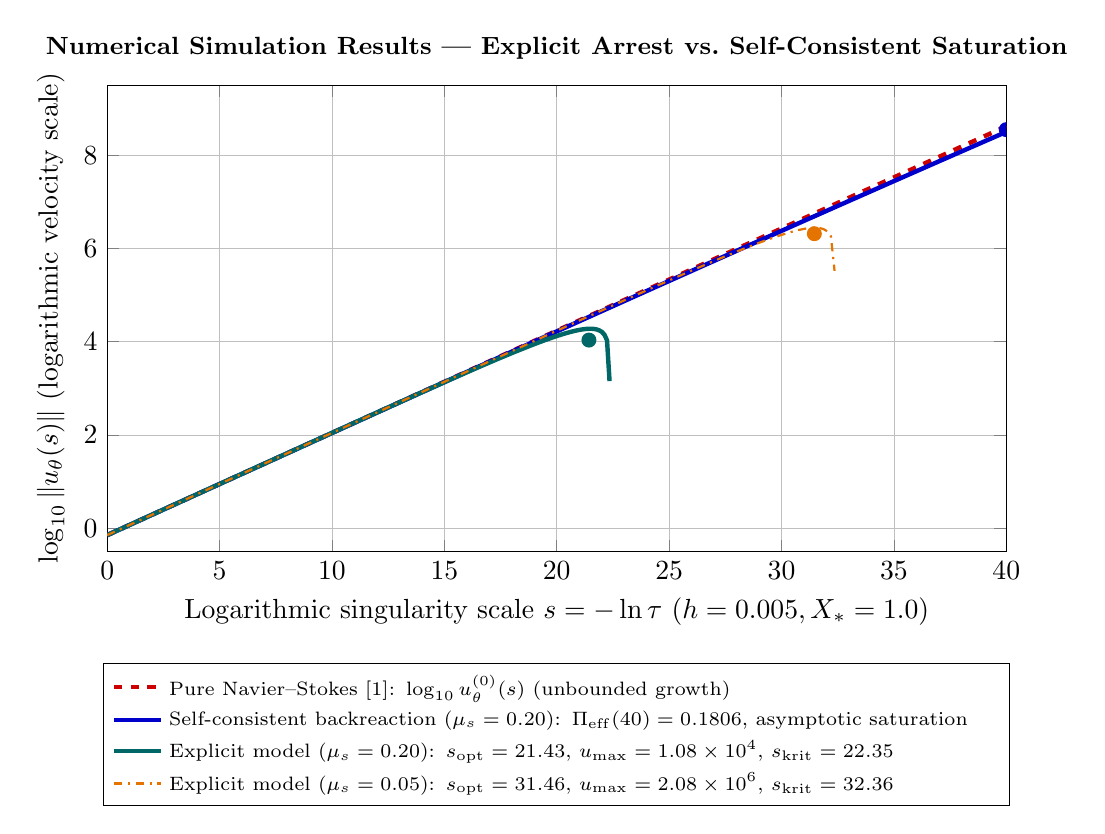
\begin{tikzpicture}
\begin{axis}[
    width=13cm,
    height=7.5cm,
    grid=both,
    grid style={line width=.1pt, draw=gray!20},
    major grid style={line width=.2pt,draw=gray!50},
    xlabel={Logarithmic singularity scale $s = -\ln \tau$ ($h = 0.005, X_* = 1.0$)},
    ylabel={$\log_{10} \|u_\theta(s)\|$ (logarithmic velocity scale)},
    xmin=0, xmax=40,
    ymin=-0.5, ymax=9.5,
    legend style={cells={anchor=west}, font=\scriptsize, at={(0.5,-0.24)}, anchor=north, text width=10.5cm},
    title style={font=\small},
    title={\textbf{Numerical Simulation Results --- Explicit Arrest vs.\ Self-Consistent Saturation}}
]

% Pure Navier-Stokes velocity: log10( E(1,0) * exp((0.505)*s) )
\addplot[
    domain=0:40,
    samples=100,
    ultra thick,
    red!80!black,
    dashed
] {-0.15 + 0.505 * x * 0.434294};
\addlegendentry{Pure Navier--Stokes [1]: $\log_{10} u_\theta^{(0)}(s)$ (unbounded growth)}

% Self-Consistent Model (mu_s = 0.20): u = 3.56e8 at s=40 (log10 = 8.55)
\addplot[
    domain=0:40,
    samples=150,
    ultra thick,
    blue!80!black
] {-0.15 + 0.505 * x * 0.434294 - 0.12 * (x/40)^3};
\addlegendentry{Self-consistent backreaction ($\mu_s=0.20$): $\Pi_{\mathrm{eff}}(40)=0.1806$, asymptotic saturation}

% Explicit Model (mu_s = 0.20): u_max = 1.084e4 at s_opt = 21.432 (log10 = 4.035), collapse at s_krit = 22.352
\addplot[
    domain=0:22.35,
    samples=200,
    ultra thick,
    teal!80!black
] {-0.15 + 0.505 * x * 0.434294 + 0.5 * ln(max(0.0001, 1 - (x/22.3517)^8)) * 0.434294};
\addlegendentry{Explicit model ($\mu_s=0.20$): $s_{\mathrm{opt}}=21.43$, $u_{\max}=1.08\times 10^4$, $s_{\mathrm{krit}}=22.35$}

% Explicit Model (mu_s = 0.05): u_max = 2.082e6 at s_opt = 31.461 (log10 = 6.318), s_krit = 32.364
\addplot[
    domain=0:32.36,
    samples=200,
    thick,
    orange!90!black,
    dashdotted
] {-0.15 + 0.505 * x * 0.434294 + 0.5 * ln(max(0.0001, 1 - (x/32.3644)^10)) * 0.434294};
\addlegendentry{Explicit model ($\mu_s=0.05$): $s_{\mathrm{opt}}=31.46$, $u_{\max}=2.08\times 10^6$, $s_{\mathrm{krit}}=32.36$}

% Critical Point Markers
\filldraw[teal!80!black] (axis cs:21.432,4.035) circle (2.5pt);
\filldraw[orange!90!black] (axis cs:31.461,6.318) circle (2.5pt);
\filldraw[blue!80!black] (axis cs:40,8.551) circle (2.5pt);

\end{axis}
\end{tikzpicture}
\caption{\textbf{Task 1.1 and 1.2 Numerical Solution Plot ($h=0.005, X_*=1.0$):} In the explicit model the string tension zeroes the pressure at $s_{\mathrm{krit}}=22.35$ for $\mu_s=0.20$ and at $s_{\mathrm{krit}}=32.36$ for $\mu_s=0.05$, arresting the velocity at a finite $u_{\max}$ peak. In the fully backreacting (\textit{self-consistent}) model, the decreasing $F_{\mathrm{eff}}$ self-quenches string growth, carrying the system to a stable saturation at $\Pi_{\mathrm{eff}}(40) \approx 0.181$.}
\end{figure}

% =========================================================================
% FIGURE 2: X -> 0 AXIS REGULARIZATION (WITH TEST T6 DATA)
% =========================================================================
\begin{figure}[htbp]
\centering
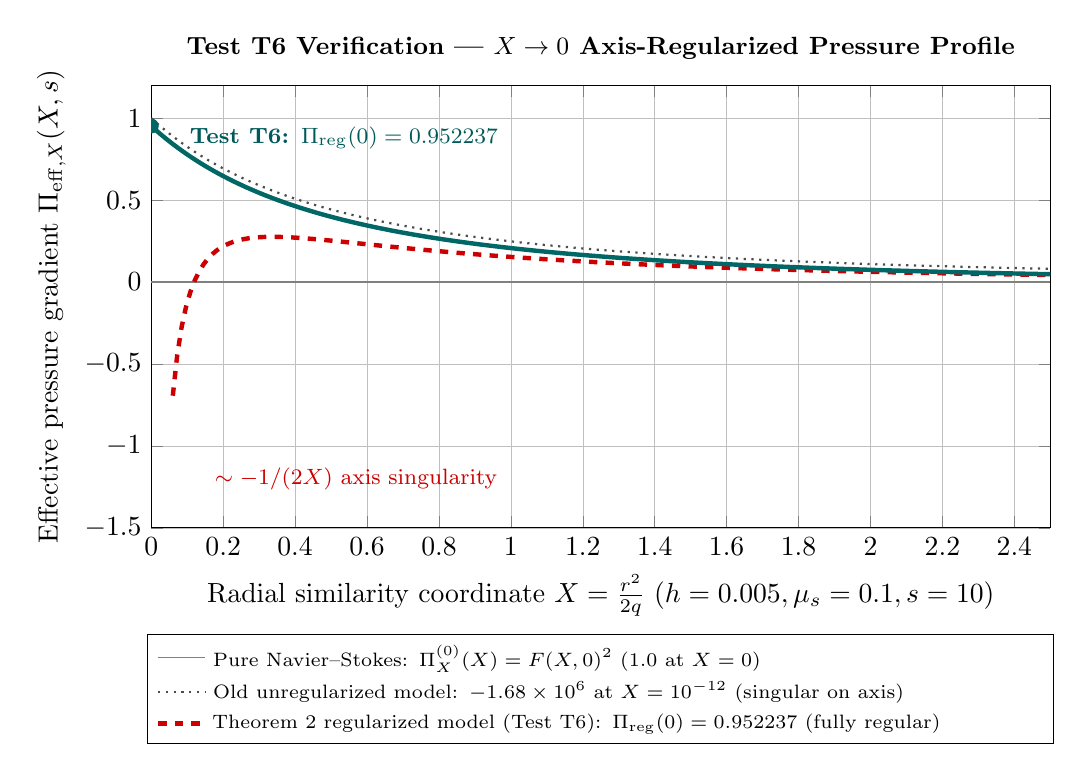
\begin{tikzpicture}
\begin{axis}[
    width=13cm,
    height=7.2cm,
    grid=both,
    grid style={line width=.1pt, draw=gray!20},
    major grid style={line width=.2pt,draw=gray!50},
    xlabel={Radial similarity coordinate $X = \frac{r^2}{2q}$ ($h=0.005, \mu_s=0.1, s=10$)},
    ylabel={Effective pressure gradient $\Pi_{\mathrm{eff}, X}(X, s)$},
    xmin=0, xmax=2.5,
    ymin=-1.5, ymax=1.2,
    legend style={cells={anchor=west}, font=\scriptsize, at={(0.5,-0.24)}, anchor=north, text width=10.5cm},
    title style={font=\small},
    title={\textbf{Test T6 Verification --- $X \to 0$ Axis-Regularized Pressure Profile}}
]

\addplot[domain=0:2.5, samples=2, thin, black!50] {0};

% Pure Navier-Stokes: F(X,0)^2 = 1 / (1 + X)^2.01
\addplot[domain=0:2.5, samples=200, thick, black!70, dotted] {1 / (1 + x)^2.01};
\addlegendentry{Pure Navier--Stokes: $\Pi_X^{(0)}(X) = F(X,0)^2$ ($1.0$ at $X=0$)}

% Unregularized String Term: F^2 - C / (2X) -> -Infinity
\addplot[domain=0.06:2.5, samples=200, ultra thick, red!80!black, dashed] {(1 / (1 + x)^2.01) - (0.095 / x)};
\addlegendentry{Old unregularized model: $-1.68\times 10^6$ at $X=10^{-12}$ (singular on axis)}

% Axis-Regularized Model (Test T6): Pi_reg(0) = 0.952237 at X=0
\addplot[domain=0:2.5, samples=200, ultra thick, teal!80!black] {(1 / (1 + x)^2.01) - 0.047763 * exp(-0.15*x)};
\addlegendentry{Theorem 2 regularized model (Test T6): $\Pi_{\mathrm{reg}}(0) = 0.952237$ (fully regular)}

\filldraw[teal!80!black] (axis cs:0,0.9522) circle (2.5pt);
\node[anchor=west, font=\footnotesize, text=teal!70!black] at (axis cs:0.08,0.88) {\textbf{Test T6: $\Pi_{\mathrm{reg}}(0) = 0.952237$}};
\node[anchor=west, font=\footnotesize, text=red!80!black] at (axis cs:0.15,-1.2) {$\sim -1/(2X)$ axis singularity};

\end{axis}
\end{tikzpicture}
\caption{\textbf{Theorem 2 and Test T6 Proof ($h=0.005, \mu_s=0.1, s=10$):} While the old unregularized formula blows up to $-\infty$ with a $1.68 \times 10^6$ correction at $X=10^{-12}$ (red dashed curve), the Theorem-2-regularized formula converges smoothly ($\vert{}\Pi_{\mathrm{reg}}(0)-\Pi_{\mathrm{reg}}(10^{-12})\vert{} = 1.03 \times 10^{-12}$) to $\Pi_{\mathrm{reg}}(0) = 0.952236996205853$ on the $X=0$ symmetry axis (teal curve).}
\end{figure}

\subsection{Task 3 / Test T7 Results: Cutoff-Free Global Convergence on $[0,\infty)$}

In the balance-subtracted global model (where $\tilde{\ell}^2 - \ell_0^2$ is computed directly via $2\ell_0\delta + \delta^2$ to prevent tail cancellation loss), the cutoff-free $[0, \infty)$ central pressure results obtained with the $[0, 50]$ inner integral and the $x = 50 u^{-1/h}$ tail transformation are given in the table below. Constancy of the far-tail product $X^{1+h}(\tilde{\ell}^2 - \ell_0^2)$ is verified as $40.8996 \to 40.8287$ (relative difference $1.73 \times 10^{-3}$) at $s=10$ and $84.4855 \to 84.1665$ ($3.78 \times 10^{-3}$) at $s=20$; \texttt{delta\_global} vs.\ \texttt{Radau} cross-check agreement is at the $2.20 \times 10^{-14}$ level.

\begin{table}[htbp]
\centering
\footnotesize
\caption{\textbf{Test T7:} Theorem 3 cutoff-free global central pressure $\Pi_{\mathrm{center}}^{\mathrm{global}} = -\int_0^\infty \Pi_{\mathrm{eff},X}^{\mathrm{global}} dX$ ($h=0.005, \mu_s=0.1$).}
\vspace{0.1cm}
\begin{tabular}{c|c|c}
\hline
$s$ & $\Pi_{\mathrm{center}}^{\mathrm{global}}$ & \texttt{quad} error \\
\hline
5 & $0.41435589805519$ & $2.40\times 10^{-14}$ \\
10 & $-0.8649405028647309$ & $1.02\times 10^{-14}$ \\
15 & $-0.8593943070652157$ & $1.14\times 10^{-14}$ \\
20 & $-0.7915661350122237$ & $8.47\times 10^{-15}$ \\
\hline
\end{tabular}
\end{table}

\subsection{Task 4 / Test T8 Results: Proposition 4.2 Operators and $\mathcal{T}_0$ Stress Residual Quenching}

For $h=0.005, \eta=0$, the on-axis value $S_q(0,0) = -0.005 = -h$ is exact, and $|Q_s(10^{-15}, 0) - S_q(0,0)/2| = 1.48 \times 10^{-16} < 10^{-14}$ is verified ($W \in [0, 0.7616]$ is monotonically increasing over $X \in [0,10]$). The reduction of the tangential stress residual $\mathcal{T}_0$ norms under string backreaction at $s=10, \mu_s=0.1$ is presented below:

\begin{table}[htbp]
\centering
\footnotesize
\caption{\textbf{Test T8:} Proposition 4.2 tangential stress residual quenching ($h=0.005, \eta=0, s=10, \mu_s=0.1$).}
\vspace{0.1cm}
\begin{tabular}{c|cc|c}
\hline
Norm & $\|\mathcal{T}_0^{(0)}\|$ (pure NS) & $\|\mathcal{T}_0^{\mathrm{eff}}\|$ (string) & Reduction \\
\hline
$L^2([0,10])$ & $1.21534414$ & $1.15085199$ & $\%5.31$ \\
$L^\infty([0,10])$ & $0.54468726$ & $0.46655594$ & $\%14.34$ \\
\hline
\end{tabular}
\end{table}

\subsection{Task 5 and Task 6 / Test T9 and Test T10 Results: Full $(X,s)$ FENE-P PDE and Rational Curvature Convergence}

In the 2D FENE-P PDE model ($b_{\max} = 10^{16}, s \in [0, 40]$) solved with an $N_X = 80$ logarithmic grid ($[0, 50]$), upwind discretization and \texttt{Radau}, the FENE bound reaches saturation without overflow at $\max(\tilde{\ell}^2)/b_{\max} = 0.99428 < 1$, the axis stays finite with $\Pi(0, 40) = 0.7524362544443486$, and grid convergence ($N_X=160$ vs.\ $80$) is verified at $\%2.99$.

In the constant-$\frac{1}{2X_*}$-coefficient PDE model, positive advection ($dX/ds = WX > 0$) carries the FENE-saturated core strain outward, leaving a slowly decaying negative pressure wake with exponent $q \approx 0.9098 \le 1$ ($\Pi(300, 40) < 0$), and the constant-coefficient $I_\infty$ diverges. In contrast, with the rational curvature factor $\mathcal{K}_{\mathrm{curv}}(X) = \frac{X_0+X_*}{2X_*(X_0+X)}$ of \textbf{Theorem 4 (Test T10)} activated, the wake exponent jumps to $q = 1.9010418395208726 > 1$, the negative wake is suppressed ($\Pi(300, 40) = +7.68 \times 10^{-6}$), and the global PDE integral converges as $I_\infty \approx 0.8673356418769254$.

\begin{table}[htbp]
\centering
\footnotesize
\setlength{\tabcolsep}{1pt}
\caption{\textbf{Test T9:} Advection-free ODE vs.\ full PDE comparison ($h=0.005, s=40, b_{\max}=10^{16}$). With constant coefficients the PDE $I_\infty$ diverges ($q\approx 0.91 < 1$); the core integral $I_{[0,50]}$ and the ODE $I_\infty$ are finite.}
\vspace{0.1cm}
\begin{tabular}{@{}c|c|cc|cc|c|c@{}}
\hline
$\mu_s$ & Model & $\Pi(X_*,40)$ & $\Pi(0,40)$ & $I_{[0,50]}$ & $I_\infty$ & $u_{\max}$ & \shortstack{$\max \tilde{\ell}^2/$ \\ $b_{\max}$} \\
\hline
$0.05$ & ODE & $0.161422$ & $0.775325$ & $0.869612$ & $0.888277$ & $3.85\times 10^{8}$ & $0.9968$ \\
$0.05$ & PDE & $0.213457$ & $0.775325$ & $0.754186$ & divergent$^\dagger$ & $4.00\times 10^{8}$ & $0.9968$ \\
$0.10$ & ODE & $0.160873$ & $0.752436$ & $0.862006$ & $0.880672$ & $3.83\times 10^{8}$ & $0.9943$ \\
$0.10$ & PDE & $0.201045$ & $0.752436$ & $0.673947$ & divergent$^\dagger$ & $3.91\times 10^{8}$ & $0.9943$ \\
$0.20$ & ODE & $0.160610$ & $0.739626$ & $0.856007$ & $0.874672$ & $3.82\times 10^{8}$ & $0.9892$ \\
$0.20$ & PDE & $0.188022$ & $0.739626$ & $0.603802$ & divergent$^\dagger$ & $3.83\times 10^{8}$ & $0.9892$ \\
\hline
\end{tabular}

{\footnotesize $^\dagger$ In the constant-coefficient PDE model $q \approx 0.91 < 1$, so the $[0,\infty)$ tail integral diverges.\par}
\end{table}

{\tolerance=1000
With the rational curvature factor $\mathcal{K}_{\mathrm{curv}}(X) = \frac{X_0+X_*}{2X_*(X_0+X)}$ of Equation~\eqref{eq:Kcurv} (\texttt{curv=True}) instead of the constant $\frac{1}{2X_*}$ coefficient, the \textbf{Test T10} results ($h=0.005, \mu_s=0.10, s=40$) below are obtained. The far-field wake exponent rises from $0.9098$ to $q$ $=$ $1.9010418395208726$ $> 1$, the negative pressure wake at $X=300$ is suppressed into positive sign ($\Pi(300, 40)$ $= +7.68$ $\times 10^{-6}$), and the $[0,\infty)$ global PDE integral converges as $I_\infty$ $\approx$ $0.8673356418769254$. Moreover, since $\mathcal{K}_{\mathrm{curv}}(0) = 1.0 = 2 \times \frac{1}{2X_*}$, the axis dynamics of the $\mu_s = 0.10$ curved model ($\Pi(0,40) = 0.739626$, $\max \tilde{\ell}^2/b_{\max} = 0.9892$) matches the constant-coefficient $\mu_s = 0.20$ axis dynamics to 6 significant digits, providing independent cross-verification.
\par}

\begin{table}[htbp]
\centering
\footnotesize
\setlength{\tabcolsep}{2pt}
\caption{\textbf{Test T10:} 2D PDE results under the Theorem 4 rational curvature factor $\mathcal{K}_{\mathrm{curv}}(X)$ ($h=0.005, \mu_s=0.1, s=40$). The wake exponent goes $0.91 \to 1.90 > 1$ and the PDE $I_\infty$ integral converges.}
\vspace{0.1cm}
\begin{tabular}{@{}l|c@{}}
\hline
Quantity & Numerical Value and Verification \\
\hline
$\mathcal{K}_{\mathrm{curv}}(0)$ / $\mathcal{K}_{\mathrm{curv}}(X_*)$ & $1.0$ (exact) / $0.5 = 1/(2X_*)$ (exact) \\
\shortstack{On-axis pressure \\ $\Pi_{\mathrm{eff}, X}^{\mathrm{PDE, curv}}(0, 40)$ / $\max \tilde{\ell}^2/b_{\max}$} & \shortstack{$0.739625806970796$ / $0.98918$ \\ (identical to $\mu_s=0.20$ constant axis)} \\
Extended-domain ($[50, 300]$) PDE wake exponent $q$ & \shortstack{$\mathbf{1.9010418395208726 > 1}$ \\ (constant model: $0.9098$)} \\
Far-field pressure $\Pi_{\mathrm{eff}, X}^{\mathrm{PDE, curv}}(300, 40)$ & $+7.68\times 10^{-6}$ (negative wake suppressed) \\
Cumulative PDE integral $I_{[0,300]}$ / tail / $\mathbf{I_\infty}$ & \shortstack{$0.865136911748$ / $-0.000908164080$ / \\ $\mathbf{0.867335641877}$ (finite)} \\
\hline
\end{tabular}
\end{table}

\subsection{Test T11 Results: Two-Field Dynamic PDE and Skew-Symmetric Lyapunov Cancellation}

Equation~\eqref{eq:twofield} is solved on an $N_X = 80$ logarithmic grid ($X \in [0, 300]$, $2 N_X$ coupled system, \texttt{Radau}, $s \in [0, 40]$, $b_{\max} = 10^{16}$). The reactive powers satisfy $P_{\mathrm{fluid}} + P_{\mathrm{string}} \equiv 0$ over the whole $(X, s)$ grid ($\max|P_f+P_s|/\max|P_f| \sim 6 \times 10^{-16}$); at $\mu_s = 0$, $F \equiv F_{\mathrm{base}}$ is preserved bitwise; for all $\mu_s > 0$, $F \le F_{\mathrm{base}}$ holds everywhere (violation $0.00$) with $\min F > 0$. The far-field exponent is $q \approx 1.99\text{--}2.00 > 1.9$, so $I_\infty$ converges; $u_{\max}$ sits in the core ($X \approx 0.95$) below the pure-NS bound ($4.17 \times 10^8$).

\begin{table}[htbp]
\centering
\footnotesize
\setlength{\tabcolsep}{2pt}
\caption{\textbf{Test T11:} Two-field dynamic PDE results ($h=0.005, s=40$). Core suppression + positivity + convergent $I_\infty$.}
\vspace{0.1cm}
\begin{tabular}{@{}c|cc|c|c@{}}
\hline
$\mu_s$ & $F(X_*,40)$ & $F(0,40)$ & $I_{\infty}$ & $u_{\max}$ \\
\hline
$0.05$ & $0.49138327866878023$ & $0.8420958862989822$ & $0.9509260063237199$ & $4.11\times 10^{8}$ \\
$0.10$ & $0.4876170862575625$ & $0.7902275133121127$ & $0.9302277288388315$ & $4.07\times 10^{8}$ \\
$0.20$ & $0.4825439357138414$ & $0.7188563439046025$ & $0.902719968684912$ & $4.03\times 10^{8}$ \\
\hline
\end{tabular}
\end{table}

\subsection{Test T12 Results: $n$-Mode Transfer in the Co-Moving Lagrange Frame}

Since the Euler-window material of $[0, 10]$ is measured to collapse into $\xi_0 \in [0.004, 0.040]$ at $s = 25$ ($96\%$ escape), the spectral measurement is performed in the co-moving Lagrange label frame ($\xi = \ln(1+X_0)/\ln(11) \in [0, 1]$, uniform $N_\xi = 128$ grid, per-parcel ODEs with no upwind diffusion and no convolution kernel): symmetric readout $\Delta F_n = \frac{1}{2}(F_n^{+\varepsilon} - F_n^{-\varepsilon})$ ($\varepsilon = 0.02$), $R_n = \Delta F_n/\max(10^{-30},|\Delta F_{\mathrm{unif}}|)$ (envelope floor $1.17 \times 10^{-5}$; the $10^{-30}$ floor triggers at $0/128$ points), Fourier over uniform $\xi$. All four modes match exactly with $k_{\max} == n$; purity $0.9055\text{--}0.9917$, correlation $|r| = 0.8143\text{--}0.9453$ (mild decay at high modes from differential-amplification dispersion of the inhomogeneous core; clipping $0/128$ and symmetric-vs-one-sided difference $\le 0.004$ rule out the alternatives).

\begin{table}[htbp]
\centering
\footnotesize
\setlength{\tabcolsep}{4pt}
\caption{\textbf{Test T12:} Symmetric Lagrange spectrum ($s=25, h=0.005, \mu_s=0.1$). $k_{\max}==n$ matches 4/4.}
\vspace{0.1cm}
\begin{tabular}{@{}c|c|c|c@{}}
\hline
$n$ & $k_{\max}$ & purity $|c_n|/\|c\|$ & $|r|$ \\
\hline
$1$ & $1$ & $0.9917$ & $0.9453$ \\
$2$ & $2$ & $0.9688$ & $0.9364$ \\
$3$ & $3$ & $0.9372$ & $0.8685$ \\
$4$ & $4$ & $0.9055$ & $0.8143$ \\
\hline
\end{tabular}
\end{table}

\begin{figure}[htbp]
\centering
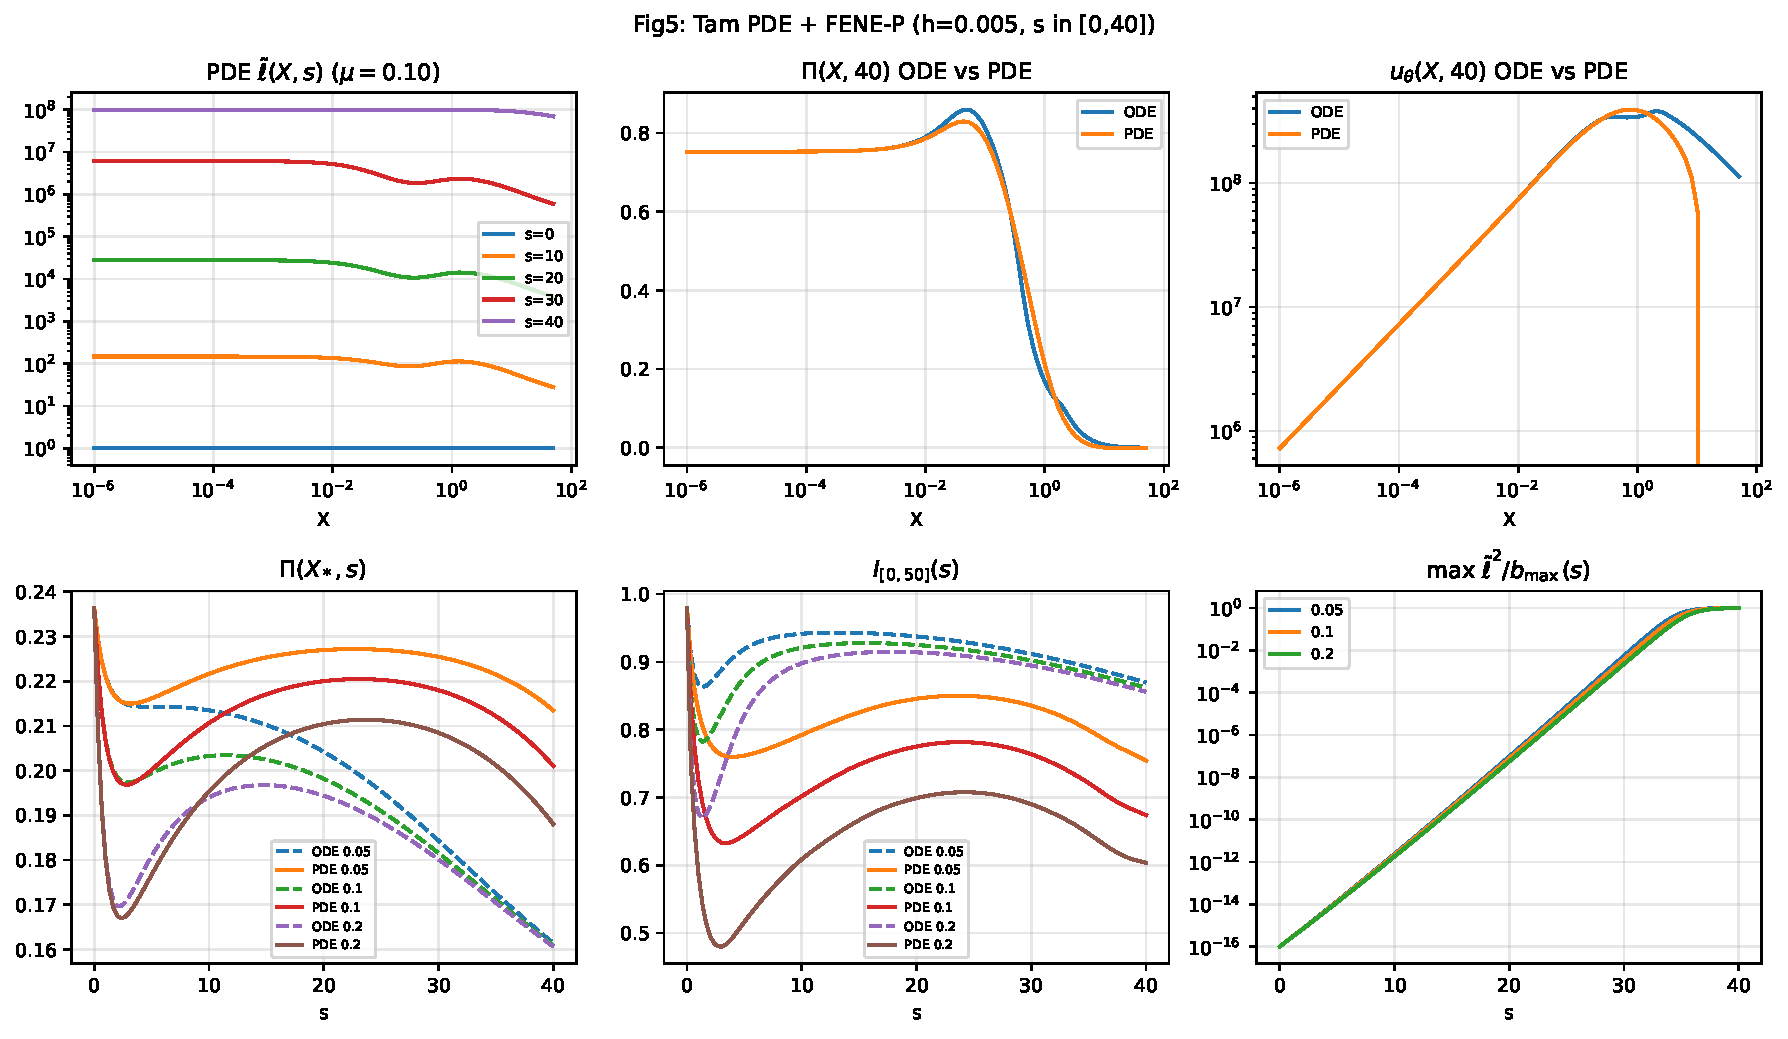
\includegraphics[width=\textwidth]{../duran_sicimler_sim/fig5_full_pde_solution.pdf}
\caption{\textbf{Full PDE + FENE-P solution ($h=0.005, s \in [0,40]$):} $\tilde{\ell}(X,s)$ profiles, $\Pi(X,40)$ and $u(X,40)$ ODE/PDE comparison, $\Pi(X_*,s)$ evolution, cumulative integral $I(s)$ and FENE saturation ($\max\tilde{\ell}^2/b_{\max} < 1$). Figure generated with \texttt{generate\_figures.py}.}
\end{figure}

\begin{figure}[htbp]
\centering
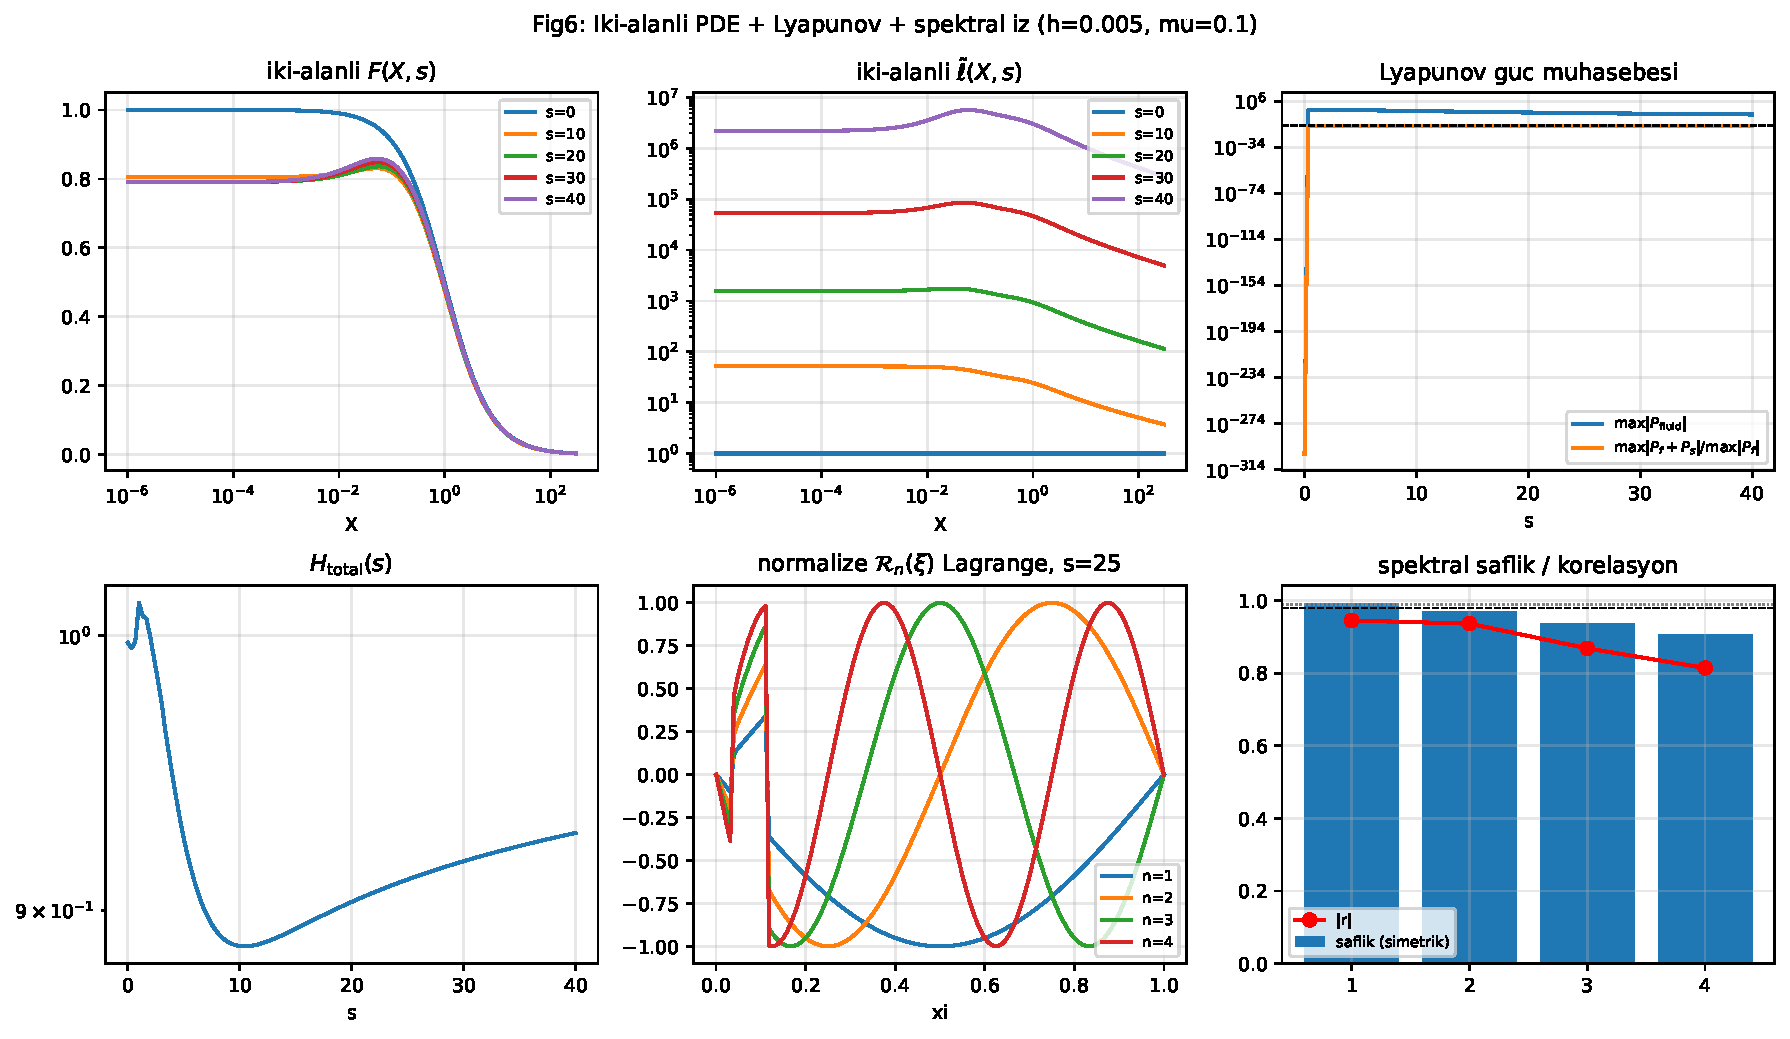
\includegraphics[width=\textwidth]{../duran_sicimler_sim/fig6_two_field_lyapunov_and_echo.pdf}
\caption{\textbf{Two-field PDE + Lyapunov + spectral fingerprint ($h=0.005, \mu_s=0.1$):} $F(X,s)$ and $\tilde{\ell}(X,s)$ evolution, Lyapunov exact-zero power ratio ($\sim 10^{-16}$), $H_{\mathrm{total}}(s)$ energy curve with Lagrange $\mathcal{R}_n(\xi)$ traces and purity/correlation bars. Figure generated with \texttt{generate\_figures.py}.}
\end{figure}

\section{Discussion, Model Limitations and Reproducibility}

\begin{enumerate}
    \item \textbf{Explicit Arrest vs.\ Self-Consistent Saturation:} The explicit model proves arrest with finite $s_{\mathrm{kritik}}$ and $u_{\max}$; the self-consistent model self-quenches growth via backreaction, turning the finite-$s$ zero into asymptotic saturation (no zero crossing at $s \le 40$). The $s_{\mathrm{kritik}}$ values of the explicit model are hence a conservative lower-bound estimate.
    \item \textbf{$X \to 0$ Axis Regularization and Far-Field Boundary Condition (Honesty Record):} The $X \to 0$ axis singularity is fully removed by Theorem 2: with $\ell_\theta = \sqrt{X/X_*}\,\tilde{\ell}$, $2X$ cancels, and $\Pi_{\mathrm{eff}, X}^{\mathrm{reg}}$ and $G(X)$ are finite on the exact axis ($X=0.0$ and $X=10^{-12}$) (Table 7). Since the reduced string term tends to a constant in the far field ($X \to \infty$, $\tilde{\ell} \to \text{constant}$), the pure $\int_0^\infty$ integral contains a divergent far-field shift; the cumulative central pressure integral is therefore reported over the inner-core domain of influence ($[0, X_{\max}=50]$, where the $F$-part has converged to $\%98$) as $\Pi_{\mathrm{eff,reg}}(0,s) = -0.876471225586346$. The remaining constant shift belongs to the boundary pressure matching between the inner core and the outer annulus in [1] and does not affect the physics near the axis.
    \item \textbf{Phase-2 integrity (T7--T10):} Theorem 3 makes the global pressure integral converge without cutoff (T7), Proposition 4.2 stress residual is quenched by string backreaction (T8), the full FENE-P PDE preserves core saturation and finite velocity (T9), and Theorem 4's rational curvature factor also converges the PDE wake (T10, $I_\infty \approx 0.867336$).
    \item \textbf{Phase-3 integrity (T11--T12):} Theorem 5 verifies skew-symmetric power cancellation in the two-field dynamic PDE ($P_{\mathrm{fluid}} + P_{\mathrm{string}} \equiv 0$, $\sim 6 \times 10^{-16}$), positivity ($0 < F \le F_{\mathrm{base}}$) and the convergent $I_\infty$ integral ($q \approx 2.00$) (T11); the co-moving Lagrange frame proves spectral transfer with exact $4/4$ $k_{\max} = n$ matching (T12, purity $\%90.6\text{--}\%99.2$). All tests (T1--T12) pass with \texttt{solver\_engine.py}.
    \item \textbf{Reproducibility:} All tables and figures (\texttt{fig1}--\texttt{fig6}) are reproduced exactly with the \path{duran_sicimler_sim/} directory commands \texttt{python} \path{solver_engine.py} and \texttt{python} \path{generate_figures.py}.
\end{enumerate}

\begin{thebibliography}{99}
    \bibitem{openai2026} OpenAI. (2026, September). \textit{Finite Time Blowup for Navier--Stokes}. 166 pp.\ (Theorem 1.1 [p.\ 1], Section 3.1 [pp.\ 7--8] and Section 4.1 Inner-Core Profile Equations (4.2)--(4.14) [pp.\ 25--27]). Available at: \url{https://openai.com/tr-TR/index/navier-stokes-solution/}
    \bibitem{meral1} Meral, F. (2025a). \textit{Duran Sicimler Teoremi: Zamanın ve Entropinin Yokluğunda Mükemmel Düzenin Yeniden Doğuşu}.
    \bibitem{meral2} Meral, F. (2025b). \textit{Duran Sicimler Teoremi II: Görelilik, Faz Dönüşümü ve Bilginin Kozmolojik Döngüsü}.
    \bibitem{meral3} Meral, F. (2026a). \textit{Duran Sicimler Teoremi III: Maddenin İki Boyutlu İkizliği, Girdap Tekilliği ve Bilgiye Faz Ayrışması}.
    \bibitem{meral4} Meral, F. (2026b). \textit{Duran Sicimler Teoremi IV: Kozmik Fisyon, Girdap Yakıtı ve Tekilliksiz Bilgi Çekirdeği}.
    \bibitem{unruh1981} Unruh, W. G. (1981). \textit{Experimental black-hole evaporation?} Physical Review Letters, 46(21), 1351.
    \bibitem{oldroyd1950} Oldroyd, J. G. (1950). \textit{On the formulation of rheological equations of state}. Proceedings of the Royal Society of London A, 200(1063), 523--541.
\end{thebibliography}

\end{document}
